\documentclass{beamer}
\usepackage{beamerthemeshadow}
\usepackage{mathtools}
\usepackage{fontspec}
\newcommand{\sam}{\textit{SAM}}
\title{\sam~ file format}
\date{}
\begin{document}
\frame{\titlepage}

\begin{frame}{\sam~ file contents}
  \begin{center}
    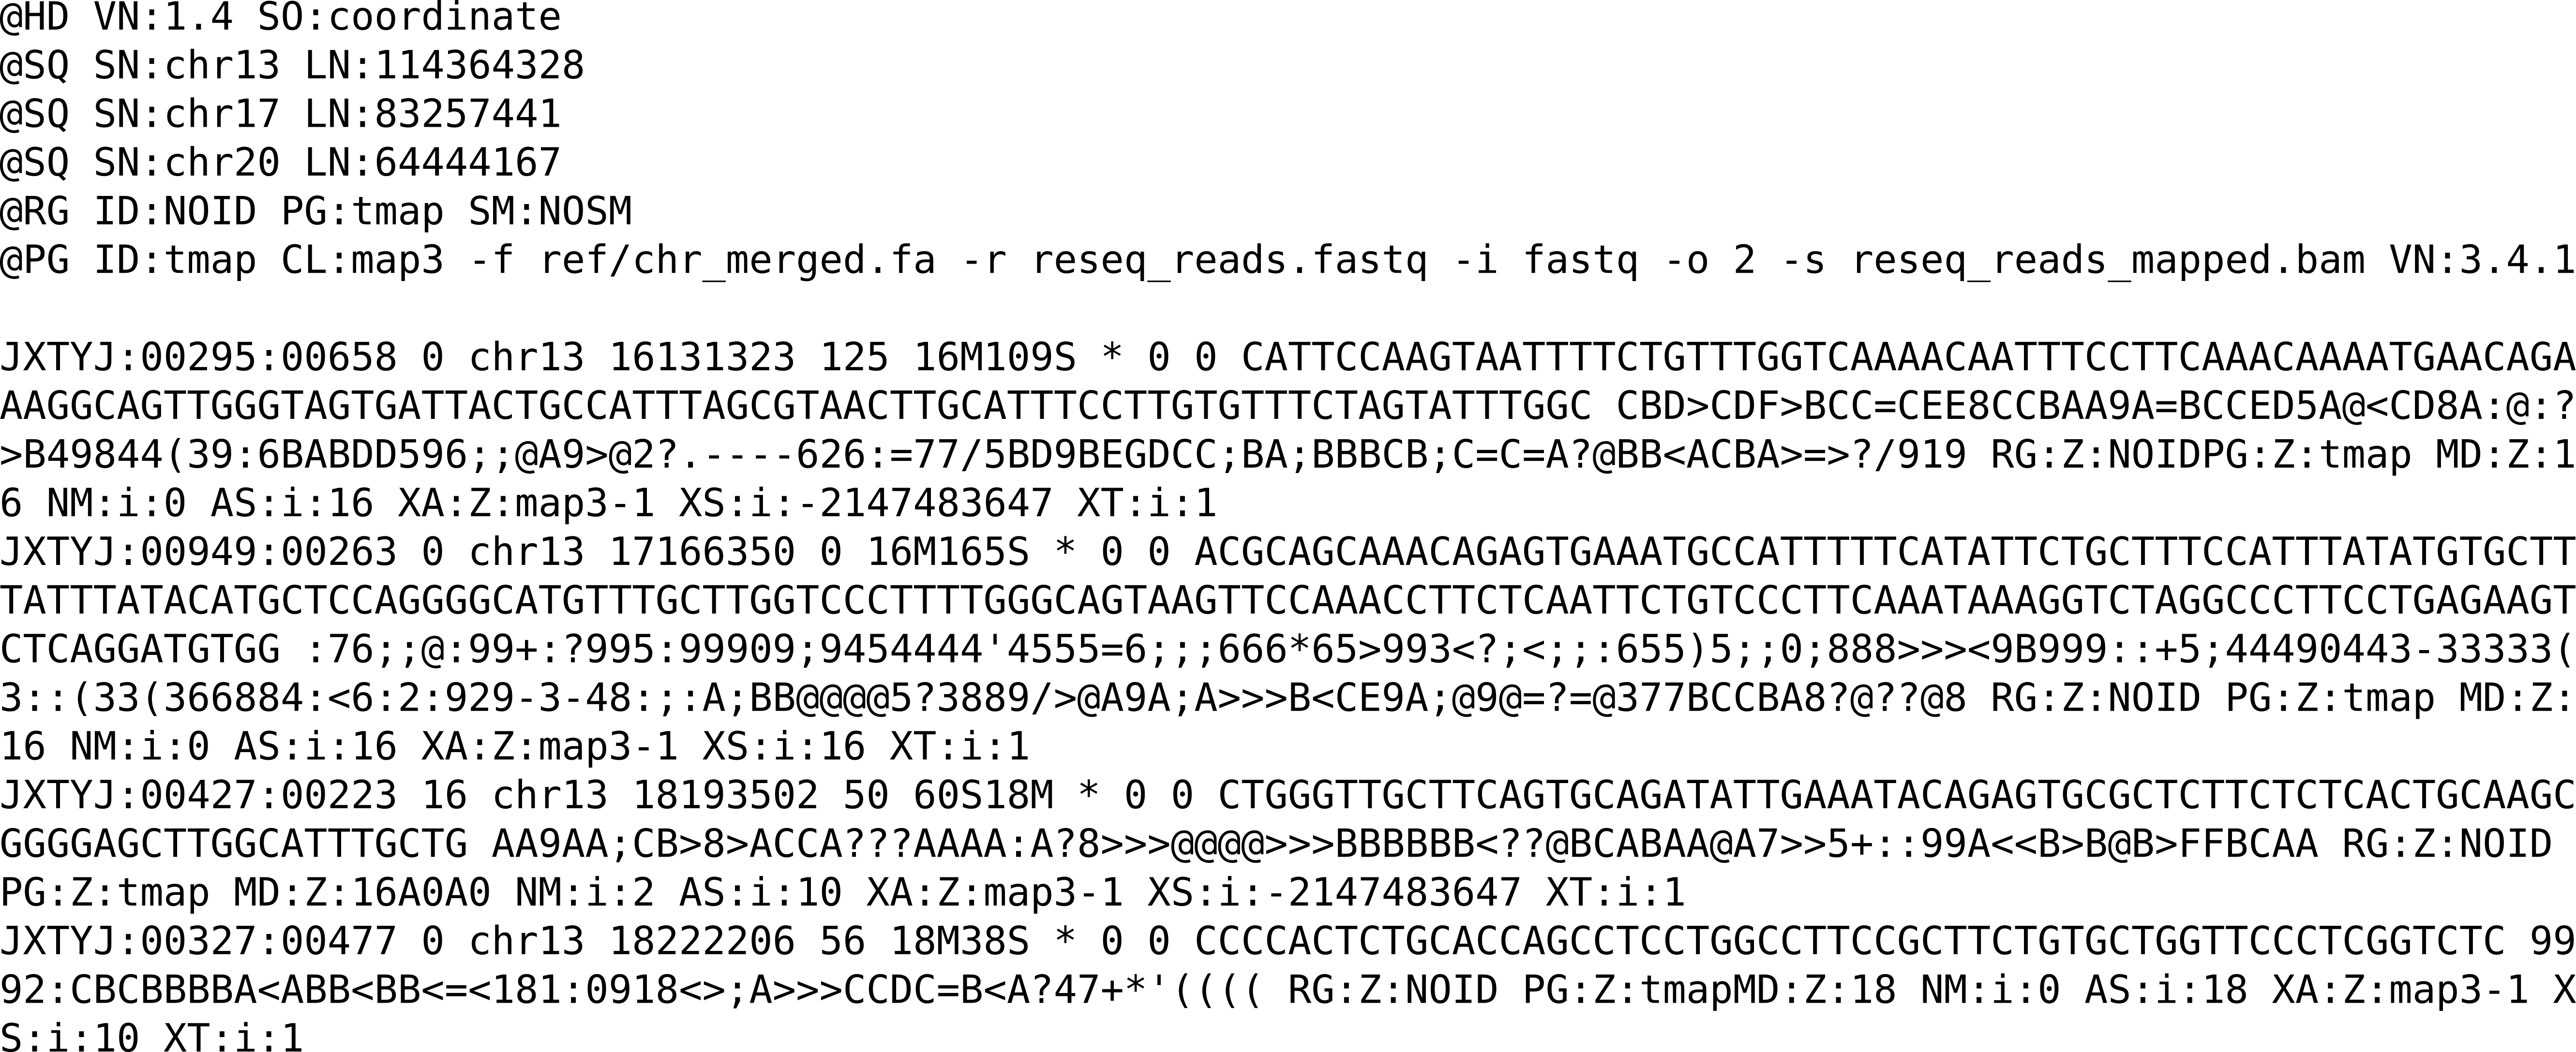
\includegraphics[width=\linewidth, keepaspectratio]{pic/sam_full.png}
  \end{center}
\end{frame}

\begin{frame}{\sam~ file contents}
  \begin{center}
    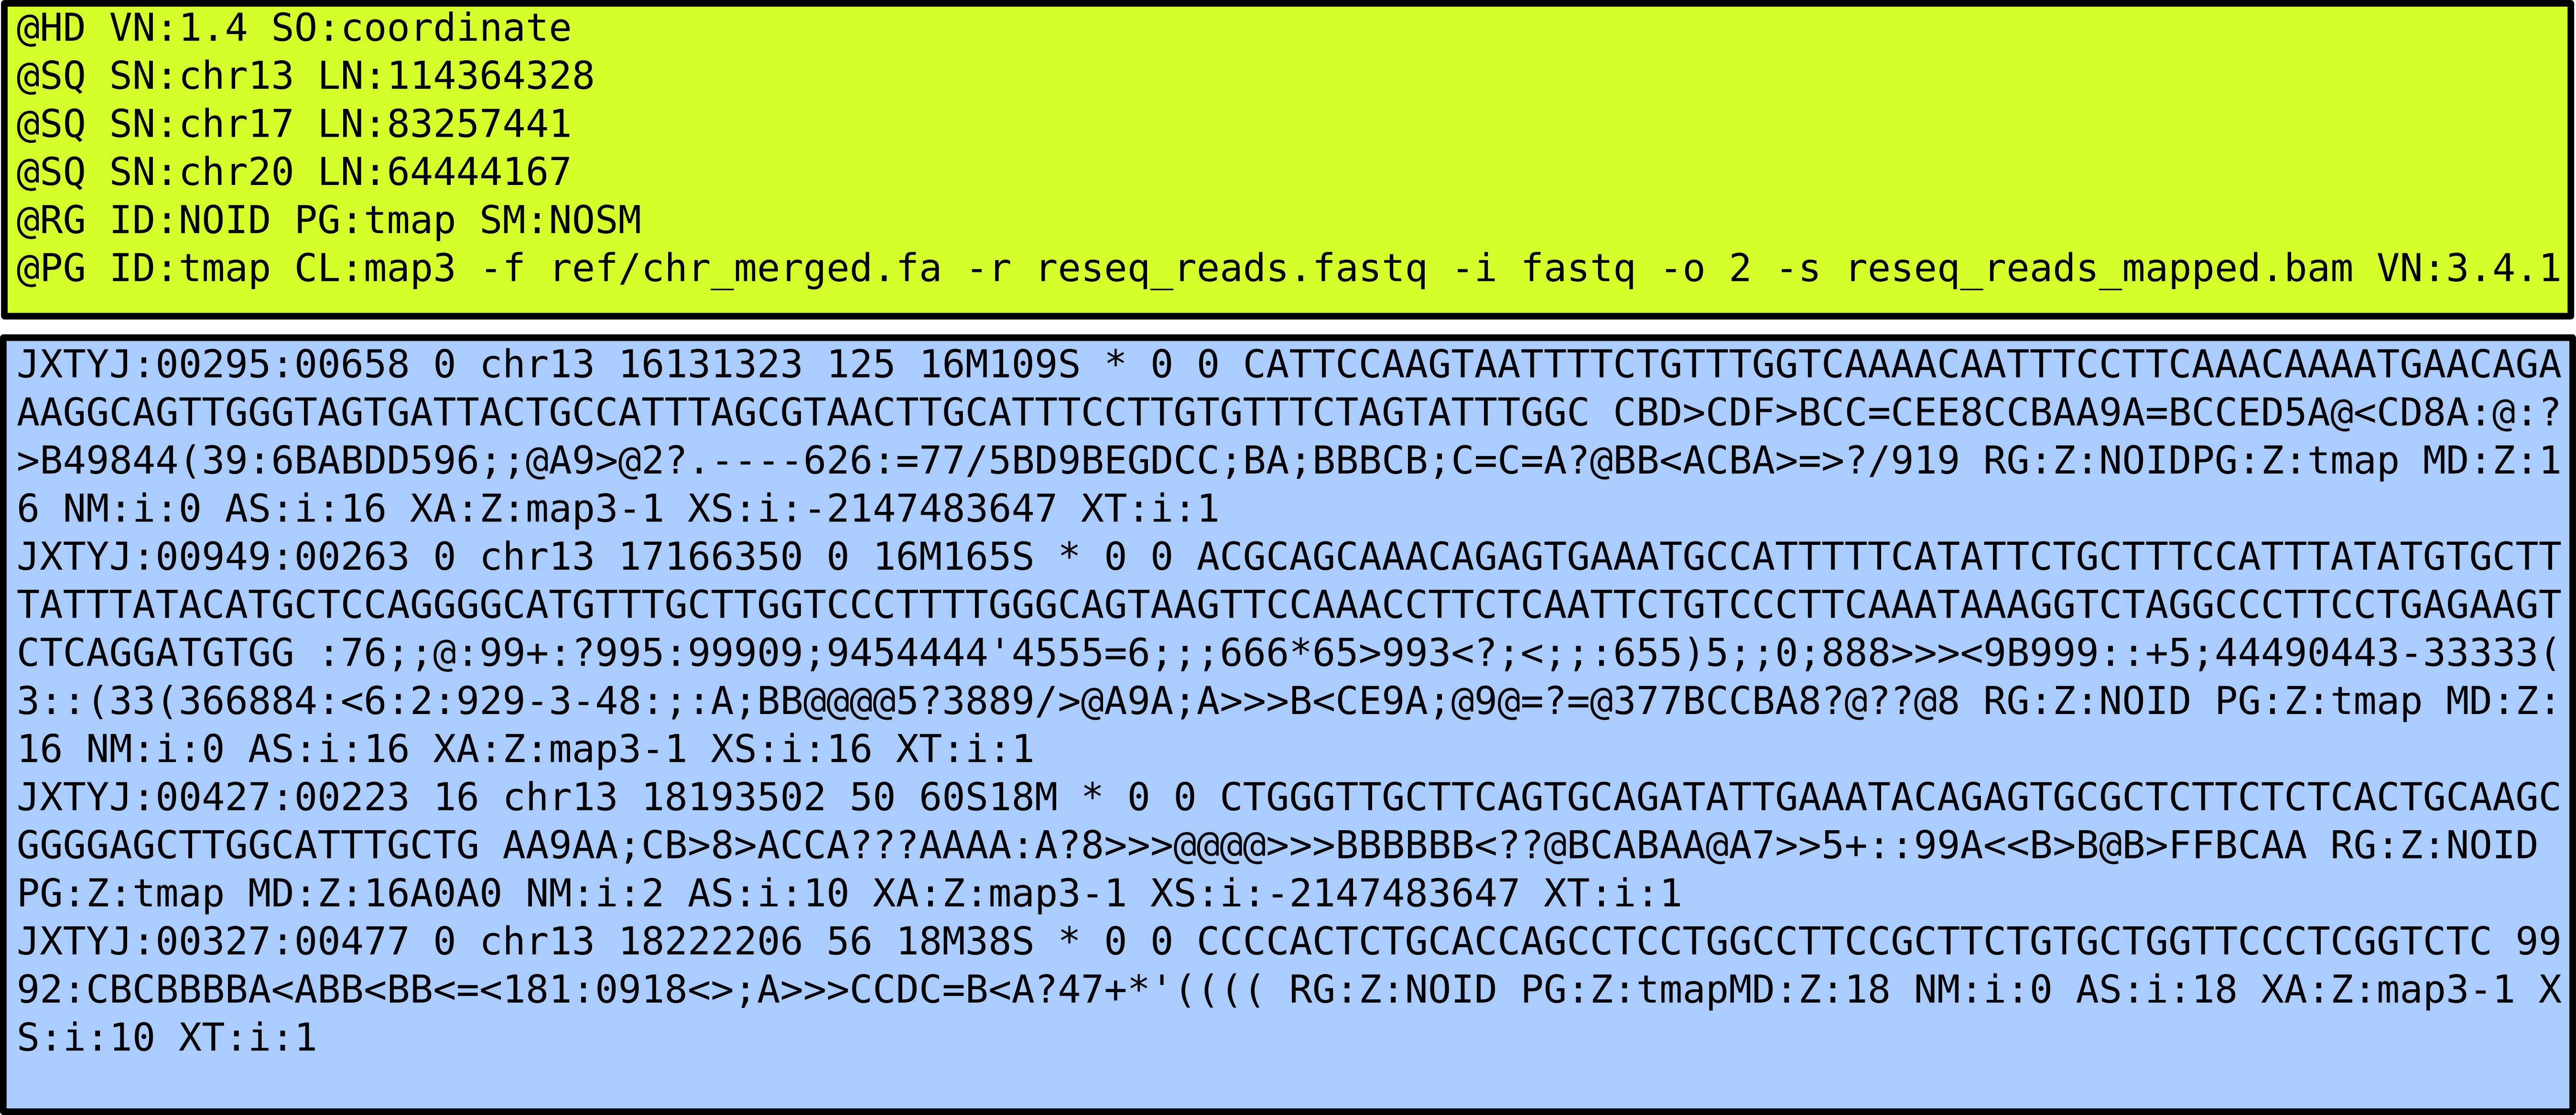
\includegraphics[width=\linewidth, keepaspectratio]{pic/sam_full_hb.png}
  \end{center}
\end{frame}



\begin{frame}{\sam~ body}
  \begin{center}
    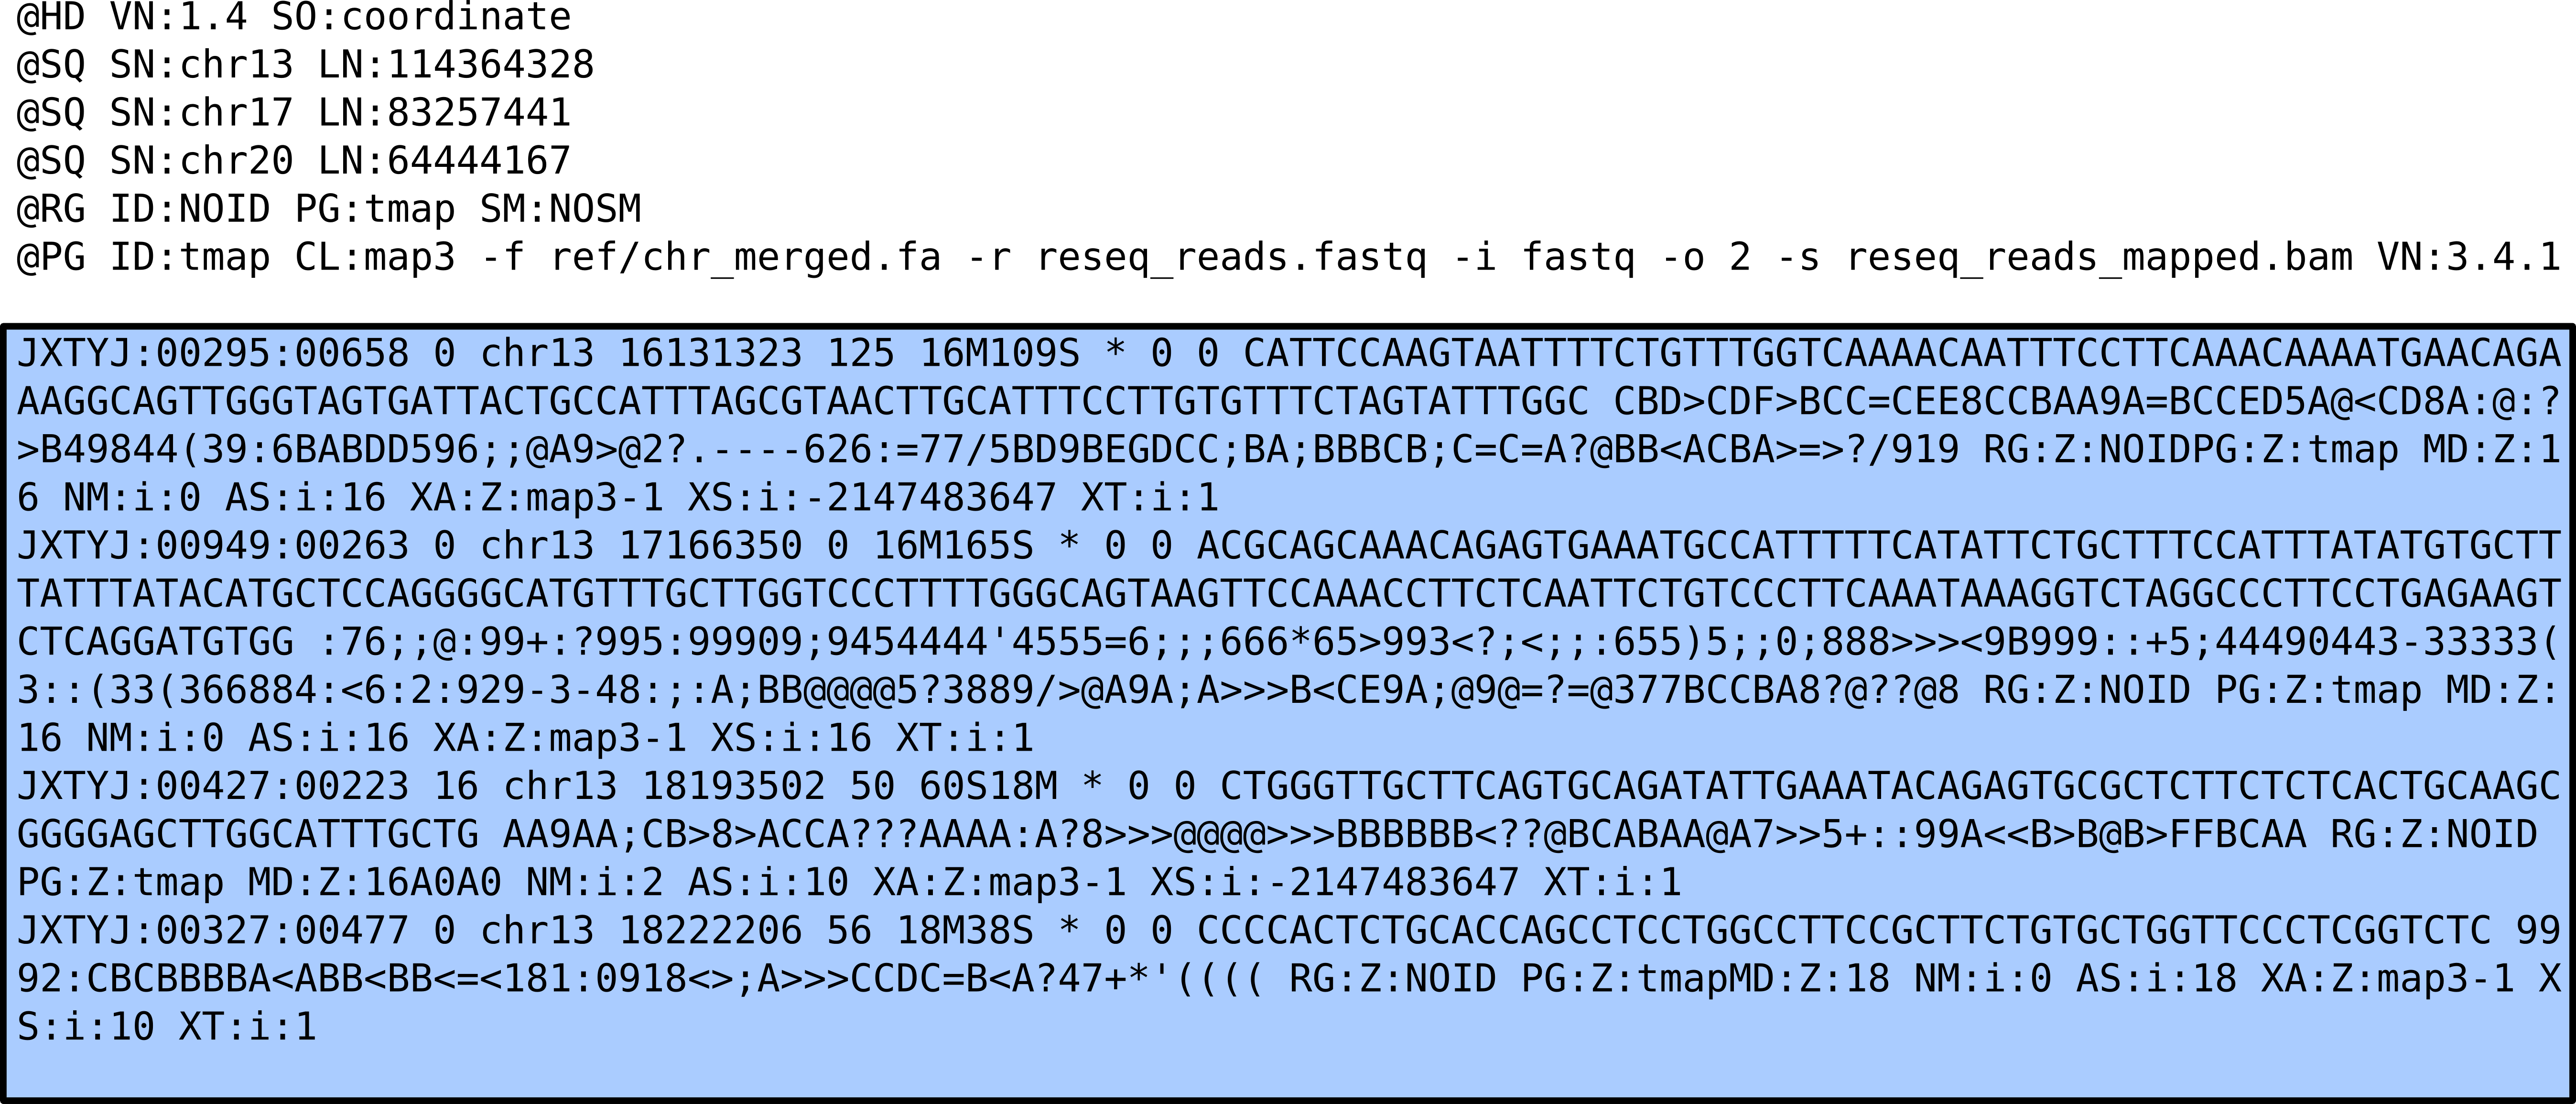
\includegraphics[width=\linewidth, keepaspectratio]{pic/sam_full_b.png}
  \end{center}
\end{frame}

%\begin{frame}{\sam~ body}
%  \begin{center}
%    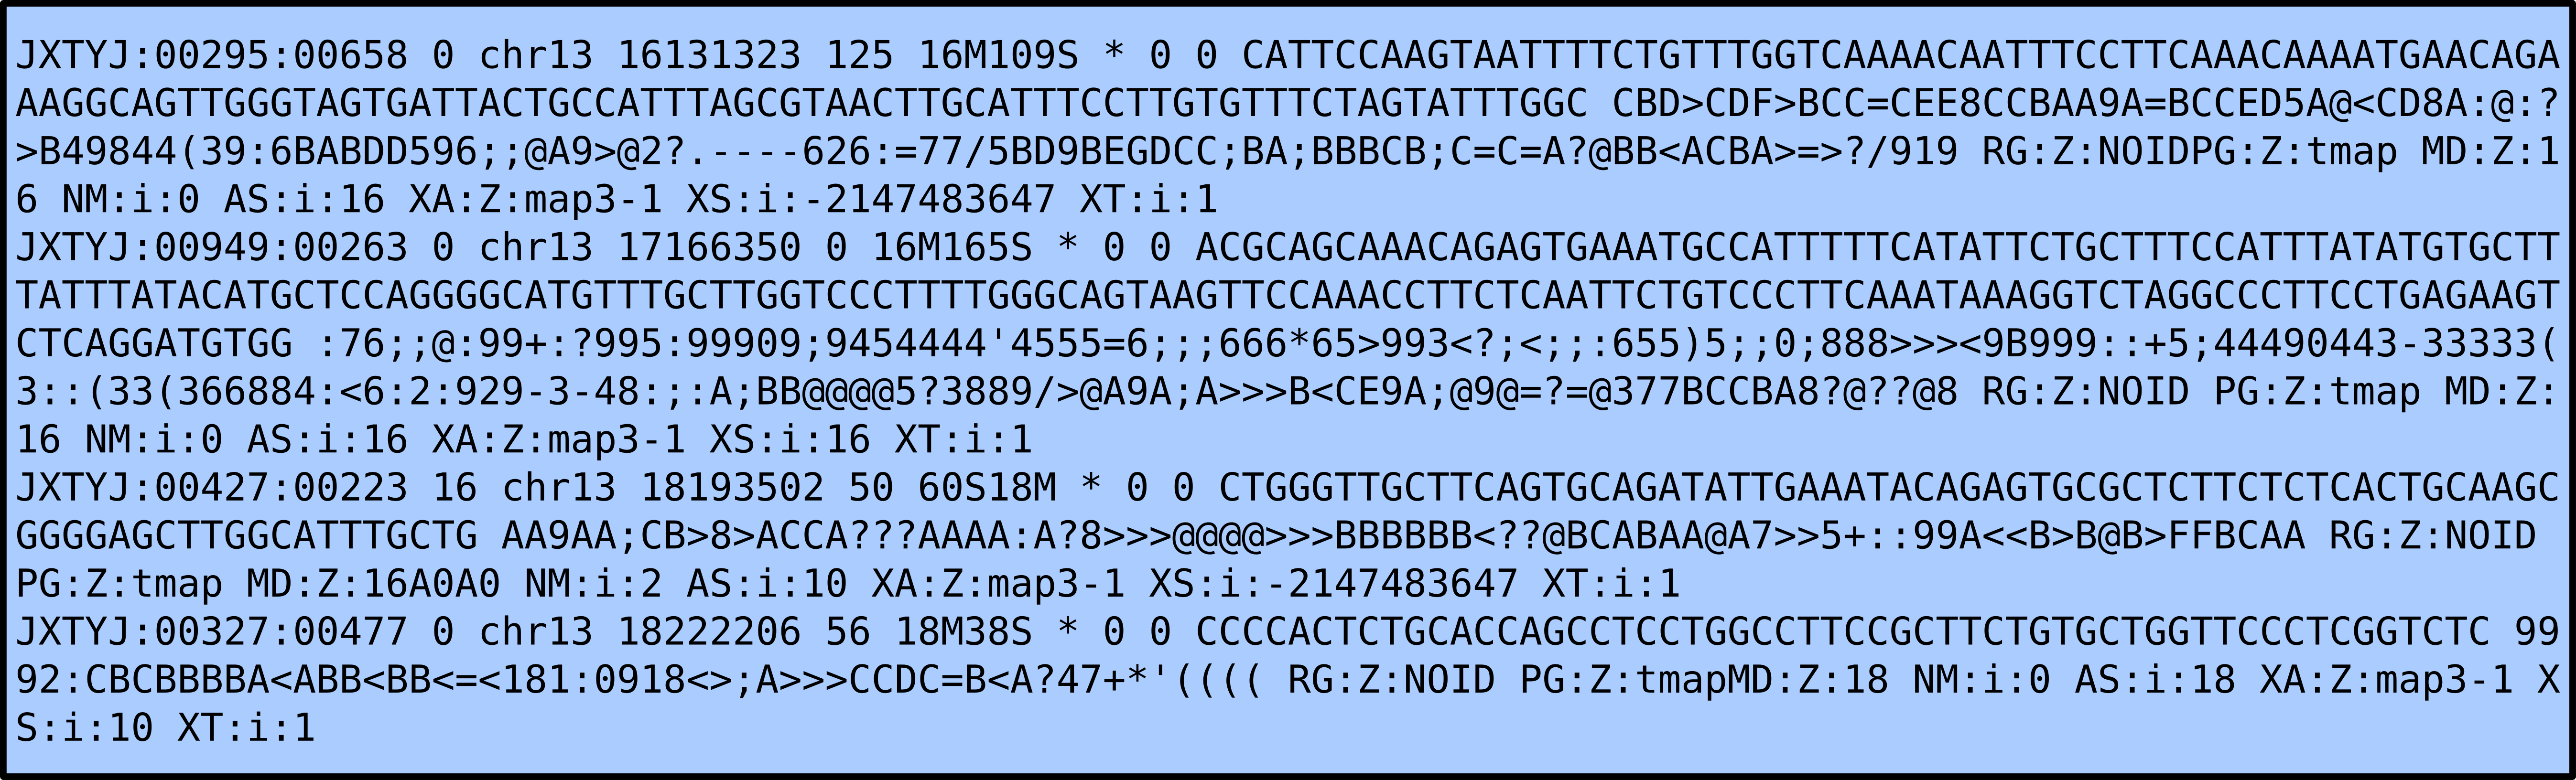
\includegraphics[width=\linewidth, keepaspectratio]{pic/sam_b.png}
%  \end{center}
%\end{frame}

\begin{frame}{\sam~ body}
  From \textit{SAM} format specification:
  \begin{tabular}{rlll}
    \hline
    {\bf Col} & {\bf Field} & {\bf Brief description} \\
    \hline
    1 & {\sf QNAME} & Query template NAME\\
    2 & {\sf FLAG} & bitwise FLAG \\
    3 & {\sf RNAME} & Reference sequence NAME\\
    4 & {\sf POS} & 1-based leftmost mapping POSition \\
    5 & {\sf MAPQ} & MAPping Quality \\
    6 & {\sf CIGAR} & CIGAR string \\
    7 & {\sf RNEXT} & Ref. name of the mate/next read\\
    8 & {\sf PNEXT} & Position of the mate/next read \\
    9 & {\sf TLEN} & observed Template LENgth \\
    10 & {\sf SEQ} & segment SEQuence\\
    11 & {\sf QUAL} & ASCII of Phred-scaled base QUALity+33 \\
    \hline
  \end{tabular}
\end{frame}



\begin{frame}{FLAG field}
  \begin{tabular}{rl}
    \hline
    Bit & Description\\
    \hline
    0x1 &  template having multiple segments in sequencing \\
    0x2 &  each segment properly aligned according to the aligner \\
    0x4 &  segment unmapped \\
    0x8 &  next segment in the template unmapped \\
    0x10 &  {\sf SEQ} being reverse complemented \\
    0x20 &  {\sf SEQ} of the next segment in the template being reversed \\
    0x40 &  the first segment in the template \\
    0x80 &  the last segment in the template \\
    0x100 &  secondary alignment \\
    0x200 &  not passing quality controls \\
    0x400 &  PCR or optical duplicate \\
    0x800 &  supplementary alignment \\
    \hline
  \end{tabular}
\end{frame}

\begin{frame}{FLAG field}
  \begin{center}
    
\includegraphics[width=\linewidth, keepaspectratio]{pic/f1.png}\\~\\
    \pause
    
\includegraphics[width=\linewidth, keepaspectratio]{pic/f2.png}\\~\\
    \pause
    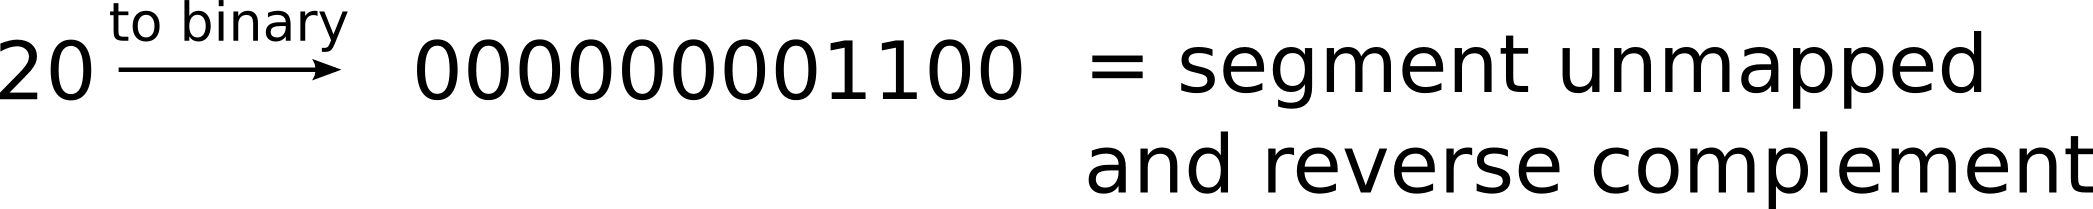
\includegraphics[width=\linewidth, keepaspectratio]{pic/f3.png}\\~\\
  \end{center}
\end{frame}

\begin{frame}{CIGAR string}
  \begin{tabular}{cl}
  \hline
  Op & Description\\
  \hline
  {\tt M} & alignment match (can be a sequence match or mismatch)\\
  {\tt I} & insertion to the reference \\
  {\tt D} & deletion from the reference \\
  {\tt N} & skipped region from the reference \\
  {\tt S} & soft clipping (clipped sequences present in {\sf SEQ})\\
  {\tt H} & hard clipping (clipped sequences NOT present in {\sf SEQ})\\
  {\tt P} & padding (silent deletion from padded reference)\\
  {\tt =} & sequence match \\
  {\tt X} & sequence mismatch \\
  \hline
  \end{tabular}
\end{frame}

\begin{frame}{CIGAR string}
  \begin{center}
    
\includegraphics[width=\linewidth, keepaspectratio]{pic/c1.png}
  \end{center}
\end{frame}

\begin{frame}{CIGAR string}
  \begin{center}
    
\includegraphics[width=\linewidth, keepaspectratio]{pic/c2.png}
  \end{center}
\end{frame}

\begin{frame}{CIGAR string}
  \begin{center}
    
\includegraphics[width=\linewidth, keepaspectratio]{pic/c3.png}
  \end{center}
\end{frame}

\begin{frame}{CIGAR string}
  \begin{center}
    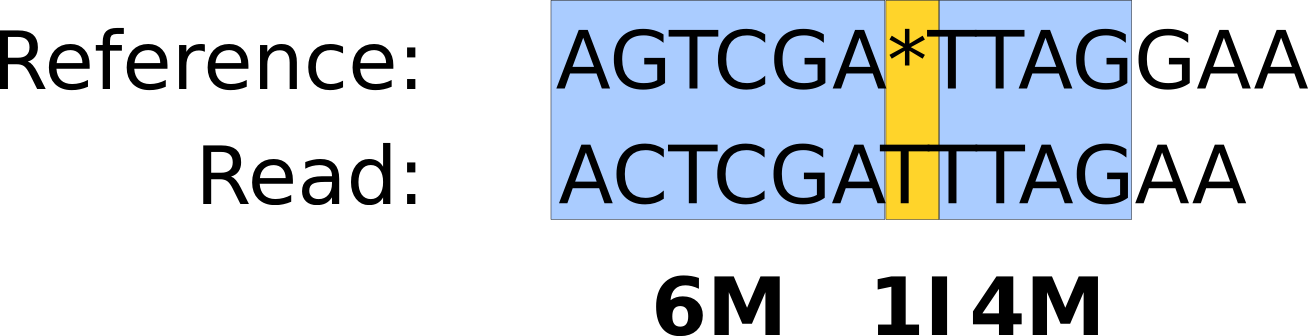
\includegraphics[width=\linewidth, keepaspectratio]{pic/c4.png}
  \end{center}
\end{frame}

\begin{frame}{CIGAR string}
  \begin{center}
    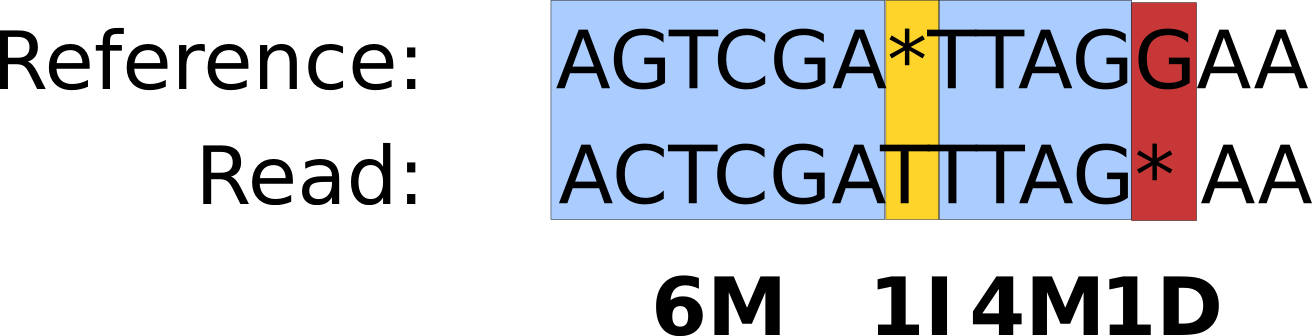
\includegraphics[width=\linewidth, keepaspectratio]{pic/c5.png}
  \end{center}
\end{frame}

\begin{frame}{CIGAR string}
  \begin{center}
    
\includegraphics[width=\linewidth, keepaspectratio]{pic/c6.png}
  \end{center}
\end{frame}

\begin{frame}{\sam~ body}
  \begin{center}
    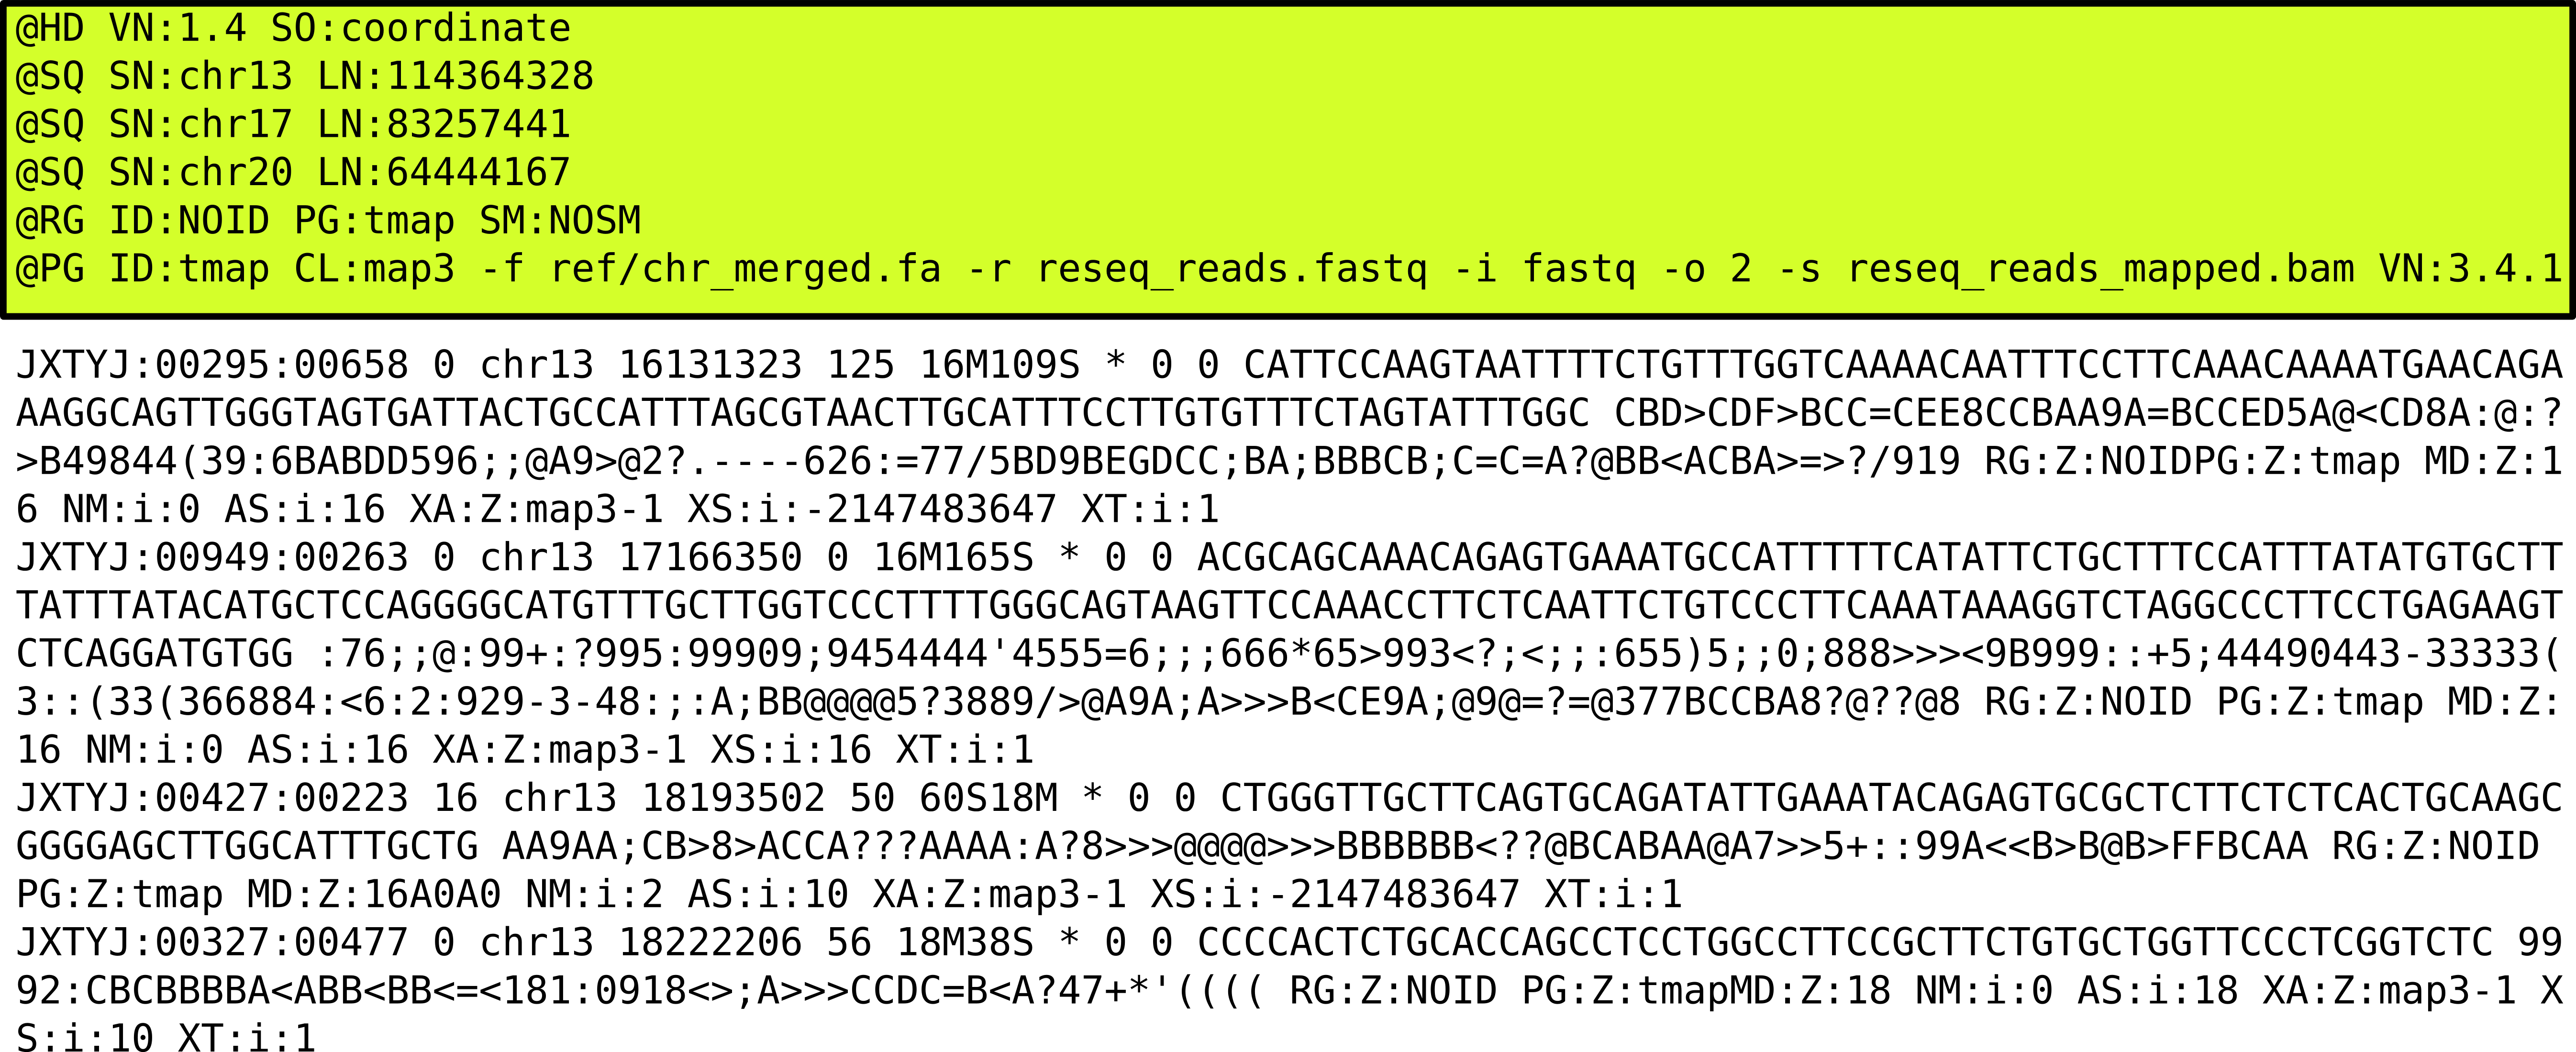
\includegraphics[width=\linewidth, keepaspectratio]{pic/sam_full_h.png}
  \end{center}
\end{frame}


\begin{frame}{\sam~ header}
  \begin{itemize}
    \item Every line starts with @ and two letter record type code
    \item Mostly follows \texttt{TAG:VALUE} format
  \end{itemize}
%\end{frame}

%\begin{frame}{\sam~ header}
  \begin{tabular}{rl}
    \hline
    Record type & Meaning\\
    \hline
    @HD & The header line. The first line if present \\
    @SQ & Reference sequence dictionary \\
    @RG & Read group\\
    @PG & Program\\
  \end{tabular}
  \begin{center}
    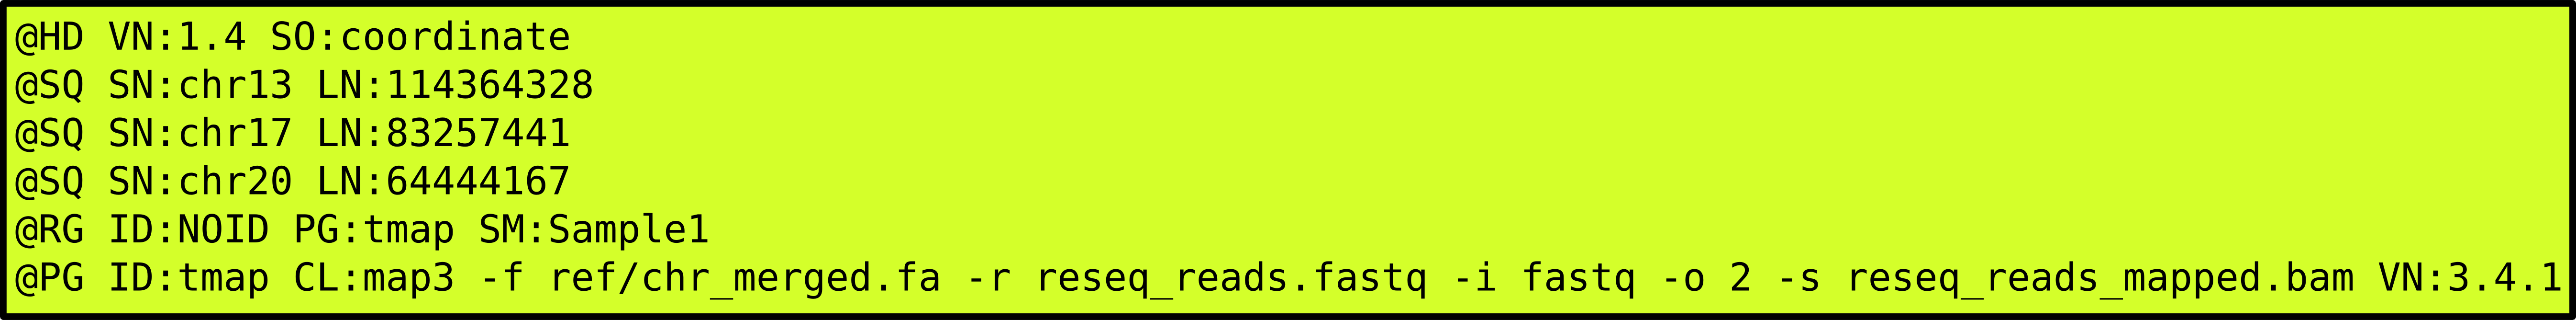
\includegraphics[width=\linewidth, keepaspectratio]{pic/sam_h.png}
  \end{center}
\end{frame}

\end{document}
